\documentclass[12pt,a4paper]{article}

\usepackage[utf8x]{inputenc}
\usepackage[english]{babel}
\usepackage{xcolor}
\usepackage{hyperref}
\usepackage{parskip}
\usepackage{graphicx}


% Path to images
\graphicspath{ {./images/} } 

% Setup for hyperrefs
\hypersetup{
    colorlinks=true,
    linkcolor=blue,
    filecolor=magenta,      
    urlcolor=blue,
}

% TODO command
\newcommand{\todo}[1]{\textcolor{red}{\textbf{[[TODO]]}} $\Rightarrow$ \textbf{#1}}
% Globally disable indentation -> package parskip
\setlength{\parindent}{0pt}

\begin{document}
    \begin{titlepage}
        \begin{center}
            \vspace*{1cm}
    
            \Large{\textbf{Project IIS}}
    
            \vspace{0.5cm}
            Monitoring of SSL connection
                
            \vspace{1.5cm}
            
            \textbf{Pavel Yadlouski (xyadlo00)}
    
            \vfill
                
            \vspace{0.8cm}
        
            Brno University of Technologies\\
            September, 2020
                
        \end{center}
    \end{titlepage}
    
    \tableofcontents
    \newpage

    \section{Introduction}
    Aim of this project is to create simple CLI application, that can monitor SSL communication.
    Here monitoring means to aggregate input file \textbf{and / or} given network interface.  
    
    \todo{For what it is needed}
    

    \section{Architecture}
    \begin{center}
        \begin{figure}[h!]
            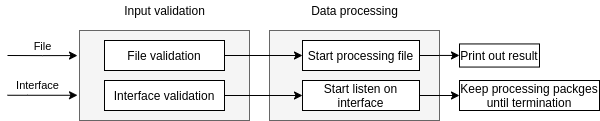
\includegraphics[scale=0.7]{sslsniff.png}
        \end{figure}
    \end{center}
    Whole program contains two main parts:
    \begin{enumerate}
        \item input validation
        \begin{enumerate}
            \item check if file exists and with supported extension
            \item check if given interface exists and can be opened for listening
        \end{enumerate}
        \item data processing
        \begin{enumerate}
            \item aggregate given file
            \item start live aggregation of incoming traffic on given interface
        \end{enumerate}
    \end{enumerate}
    The result of file aggregation is written to the standard output as soon as it is
    ready. If interface was given, than program would run and print out updates. 
    Here "updates" means when new package is came, check if it corresponds to one 
    of already created connections. If entry \textbf{exists}, then necessary info would be 
    extracted from package, added to corresponding connection and new values of 
    this connection will be written to standard output. In connection does \textbf{not exist},
    then new entry would be inserted to list of all connection and also this update would 
    be written to standard output.

    \todo{Multithreading}\\
    \todo{How processing of TLS headers works
        \begin{enumerate}
            \item structure for extensions
        \end{enumerate}
    }

    \subsection{File aggregation}
    
    \subsection{Interface aggregation}
    
    
    \section{Implementation}
    Program contains two parts: checking of input parameters and package aggregation by itself.
    First part presents in file \textit{sslsniff.c}. Also setup functions for aggregation are 
    called there. Second part is represented in file \textit{functions.c}.

    \todo{Add code snipets of used structures}\\
    \todo{Structure to capturing connections}\\
    \todo{How duration is found}


    \section{Literature}

    \todo{Refere to \href{https://www.cloudflare.com/learning/ssl/what-happens-in-a-tls-handshake/}{web page} about SSL handshake}\\
    \todo{RFC for SSL/TLS headers} \\
    \todo{TCPDump site}

\end{document}